\chapter{Estado de la cuestión}
\label{chap:antecedentes}

\drop{E}n este capítulo se presenta una visión general sobre los conceptos teóricos y técnicos que sirven como base para la elaboración de este documento, contribuyendo a su base tecnológica y de conocimiento.

Se desea resaltar que el presente proyecto no versa sobre el desarrollo de una aplicación software, sino que el objetivo principal del mismo, como ya se ha mencionado, es realizar un proceso de analisis y mejora de la metodología de \ac{Madrija} para implantar un sistema de integración continua, por lo tanto, se realizará un recorrido analizando la contribución, posibilidades y aportaciones relevantes a las diferentes áreas de la informática que trata \ac{Madrija}, justificando así la utilidad de desarrollar el presente trabajo.

\section{Ingeniería del Software}

La ingeniería del software es una disciplina, o área, de la informática\cite{Pressman1988}, que ofrece métodos y técnicas para desarrollar y mantener software de calidad que resuelven problemas de todo tipo.

La ingeniería del software trata áreas muy diversas de la informática, tales como construcción de compiladores o sistemas operativos. Y, la que más concierne para este trabajo, la integración continua, abordando todas las fases del ciclo de vida del desarrollo de cualquier tipo de sistema de información.

\section{ISO 12207}
Tal y como se explica en el capítulo 1, \ac{Madrija} utiliza la \ac{ISO} 12207\cite{ISO_12207} para gestionar su ciclo de vida de desarrollo, \ac{ISO} 12207 es el estándar que describe la arquitectura de los procesos de ciclo de vida del software de la organización \ac{ISO}. La norma no describe detalles sobre como llevar a cabo estos procesos ni las tareas que componen los mismos. Además, establece un marco común para los procesos del ciclo de vida del software, con una terminología bien definida, que puede ser referenciada por la industria del software. Contiene procesos, actividades y tareas que se van a aplicar durante la adquisición de un producto o servicio de software y durante el suministro, desarrollo, operación, mantenimiento y eliminación de productos de software.

Por lo que \ac{Madrija} ha implantando su propia metodología de desarrollo y dentro de dicha metodología se pretende implantar el sistema de integración continua para mejorarla.

\section{Inicios de la integración continua}

\ac{XP} es una metodología de desarrollo de software que enfoca a todo el equipo en objetivos comunes y alcanzables\cite{XP}. Utilizando los valores y principios de \ac{XP}, los equipos aplican prácticas apropiadas de XP en su propio contexto. Los equipos \ac{XP} producen software de calidad a un ritmo sostenible.

\ac{XP} surgió como una nueva manera de encarar proyectos software\cite{ReglasPracticasXP}, proponiendo una metodología basada, en esencia, en la simplicidad y agilidad. Las metodologías de gestión de proyectos tradicionales (ciclo de vida en cascada, en espiral, etcétera) aparecen comparadas con \ac{XP}, como metodologías pesadas y poco eficientes. La crítica más frecuente a estas metodologías “clásicas” es que son demasiado burocráticas.

%\begin{figure}[!h]
%\centering
%   
\includegraphics[width=12cm]{CicloVida_XP.png}
%\caption{Ciclo de \ac{XP}\cite{Foto_XP}}
%\end{figure}

\begin{figure}[!h]
\centering
   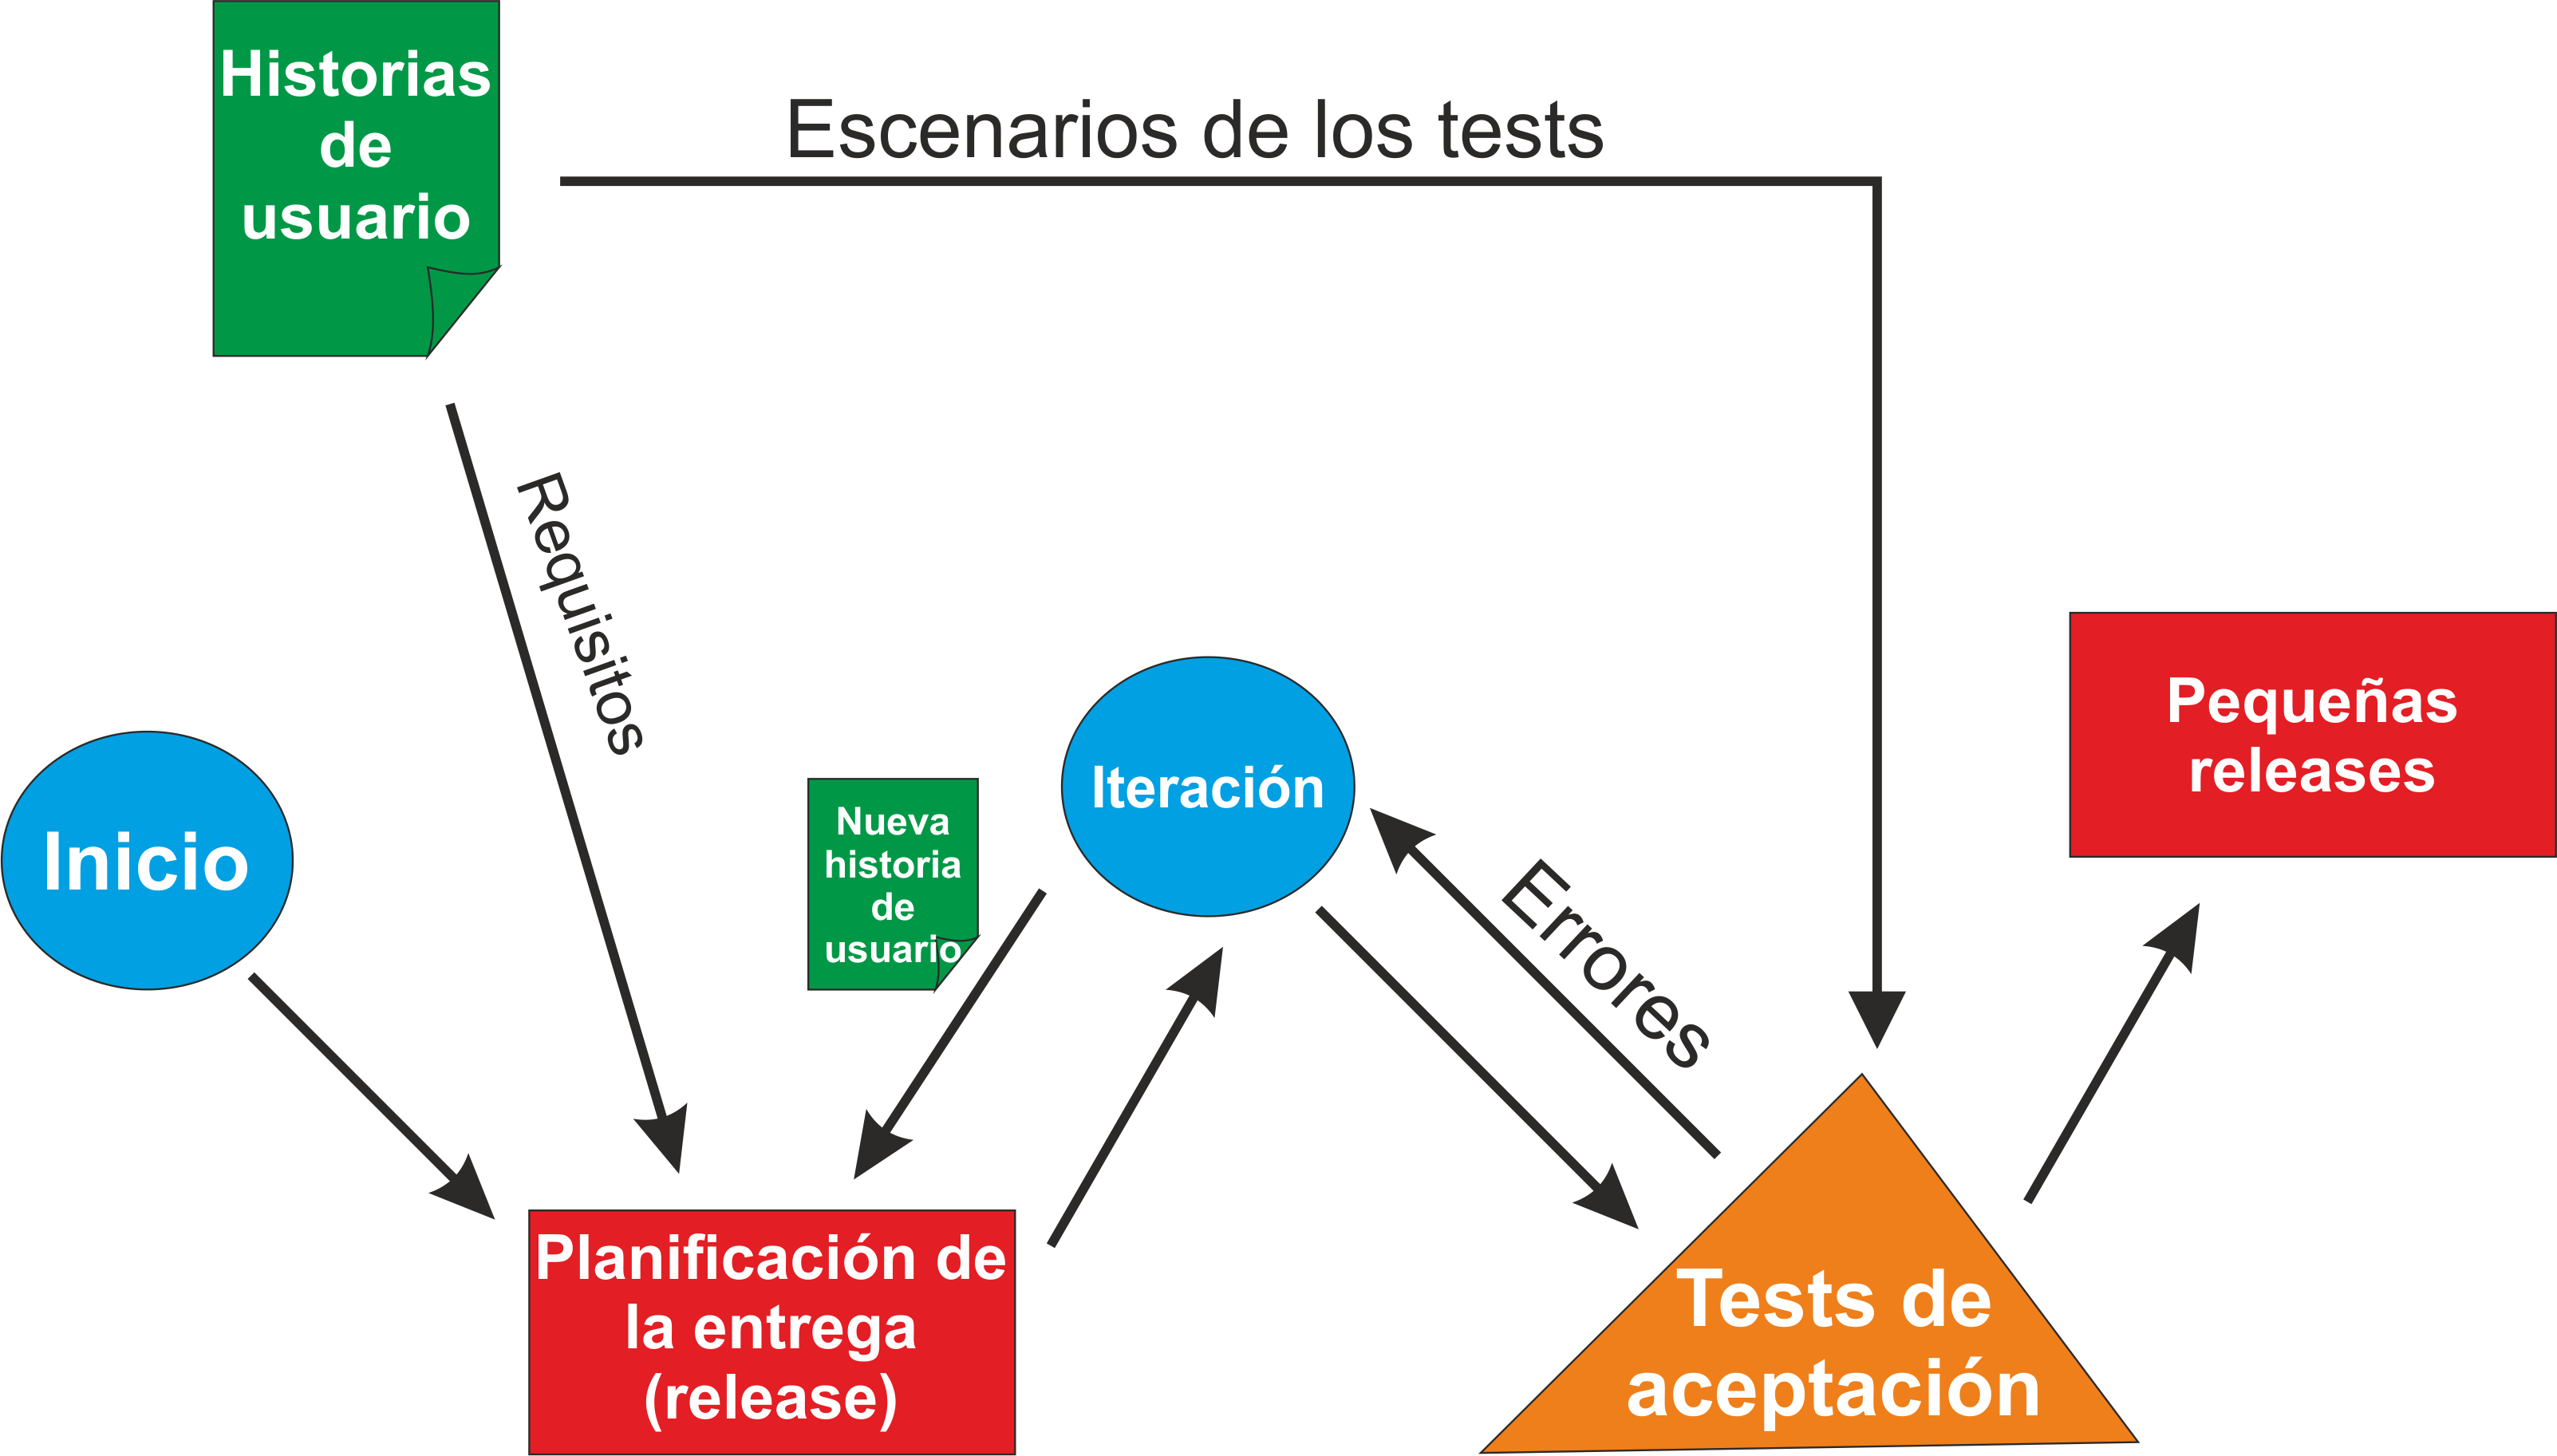
\includegraphics[width=15cm]{Ciclo_XP.png}
\caption{Ciclo de \ac{XP}\cite{Foto_XP}}
\end{figure}

Al desarrollarse \ac{XP}, se desarrollaron una serie de buenas prácticas entre las que destacan \ac{TDD}, \textit{pair programming}, testing continuo o la integración continua, ya que los equipos \ac{XP} realizan numerosos \textit{commits} varias veces por día.
El beneficio de esta buena práctica de \ac{XP} se observa en esos proyectos, donde la construcción se realiza semanalmente (o incluso mensualmente), y que, con frecuencia, terminan en un ``infierno de integración'', donde el código desarrollado no funciona y ningún desarrollador conoce el motivo.

\clearpage

Uno de los principales motivos por los que ocurren estas situaciones es la integración infrecuente de código en el repositorio, es decir, la integración infrecuente consiste en no realizar, al menos diario, la integración de código fuente que posee el desarrollador en local al repositorio donde trabaja todo el equipo de desarrollo, realizar un \textit{build} de ese código y ejecutar las pruebas necesarias para comprobar la integración de los módulos, artefactos y dependencias.

La integración infrecuente lleva a problemas serios en proyectos software\cite{LeonardoDeSeta}:
\begin{enumerate}
\item Aunque la integración continua es crítica para desarrollar un buen software, los equipos de desarrollo no la practican a menudo, delegando estas tareas a personas que no están familiarizadas con el sistema completo.
%\clearpage
\item La integración infrecuente suele generar código con errores. En el momento de integrar, aparecen problemas que no se detectaron ni ocurrieron cuando se realizaron las pruebas al software sin integrar.
\item Los procesos de integración infrecuentes generan largos periodos de ``congelación del código''. La congelación de código consiste en, que por largos períodos de tiempo, los programadores no pueden agregar nuevas características al software, puesto que no van a apreciarse los cambios realizados, dado que no están reparados los errores en el sistema, el sistema no está listo, dado que al realizar \textit{commit} lo más normal es que surjan conflictos y no compile el código.
\end{enumerate}

\section{Integración continua}

Dentro de la ingeniería del software, se encuentra la integración continúa, desarrollada de la mano de Martín Fowler\cite{IC}, integración continua es una práctica de desarrollo de software donde los miembros de un equipo integran su trabajo con frecuencia, en general, cada persona integra su trabajo, al menos una vez al día, lo que conlleva a múltiples integraciones por día. Cada integración se verifica mediante una compilación automatizada, incluidas las pruebas, con el objetivo de detectar errores de integración de manera rápida. Muchos equipos encuentran que este enfoque reduce significativamente los problemas de integración y permite desarrollar software de manera cohesiva y más rápida.

Por consiguiente, un entorno de integración continua permite la reducción de riesgos y la realización de tareas repetitivas, alcanzando un alto grado de automatización de los procesos involucrados en el desarrollo software, permitiendo la generación de software listo para desplegar.

La idea de integración continua nació de la mano de Martin Fowler tal y como se ha dicho antes, pero no fue el único, dado que parte de los autores del manifiesto ágil y otros ingenieros apoyaron la propuesta de Fowler:

\clearpage

%\section{Principales contribuciones para la integración continua}

\begin{itemize}
\item \textbf{Martin Fowler:} renombrado autor, consultor de software, orador y precursor de la integración continua, aporta dos décadas de experiencia ayudando a las empresas a utilizar tecnología orientada a objetos para sistemas de información críticos. Es uno de los autores del \textit{Manifiesto para el Desarrollo de Software Ágil}, escritor de libros sobre desarrollo de software y orador de gran prestigio en conferencias internacionales.

\item \textbf{Kent Beck:} ingeniero de software estadounidense\cite{XP2}, es uno de los creadores de las metodologías de desarrollo de software \ac{XP} y \ac{TDD}, incluyó la integración continua como una de las buenas prácticas dentro de \ac{XP}.

\item \textbf{Paul Duvall:} CTO en Stelligent. Experto en soluciones de entrega continua e integración continua en Amazon Web Service. Trabaja aplicando la integración continua con clientes como Sony Pictures Entertainment, Nutrisystem, Macy's, grandes compañías financieras, el gobierno de los Estados Unidos de América, Symantec, HP y Cardinal Health.\\Autor del libro ganador del premio Jolt Product Excellence 2008 "Integración Continua: Mejorando la Calidad del Software y Reduciendo el Riesgo", orador en las principales conferencias de software sobre integración continua.

\end{itemize}

\begin{figure}[!h]
\centering
   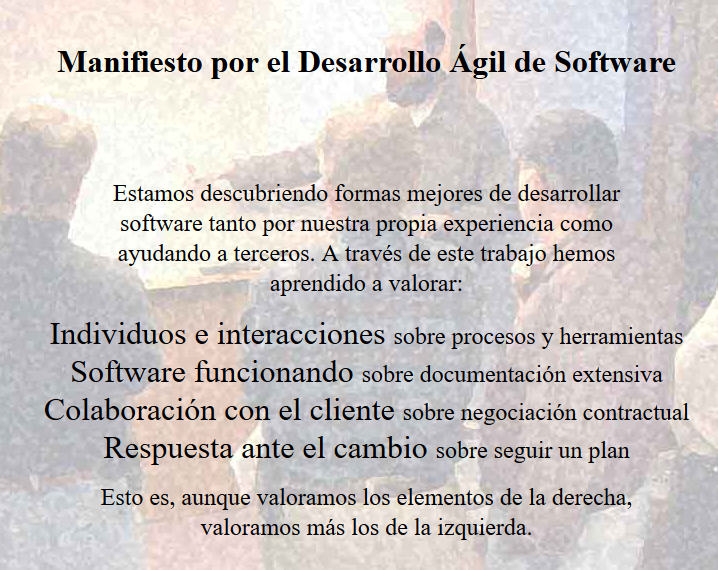
\includegraphics[width=12cm]{Manifiesto_Agil.PNG}
\caption{Algunos principios del \textit{Manifiesto para el Desarrollo de Software Ágil} \cite{TheAgileManifesto}}
\end{figure}

Todos ellos tienen en común que apoyaron el nacimiento y la evolución del desarrollo ágil, utilizando sus prácticas, entre las que destaca la integración continua.

%\section{Enfoques}

\subsection{Desarrollo ágil}

A través del estudio e investigación, se deduce que una metodología ágil es una alternativa fiable a una metodología tradicional. Las metodologías ágiles desarrollan software de manera iterativa e incremental. Las metodologías ágiles se basan en \textit{El Manifiesto Ágil}\cite{TheAgileManifesto}, documento donde se publicaron ``los pilares'' del desarrollo ágil, por ejemplo, \textit{``Individuos e interacciones sobre procesos y herramientas''}, \textit{``Software funcionando sobre documentación extensiva''}, \textit{``Respuesta a un cambio sobre seguir un plan''}, etcétera.

A menudo, las experiencias reportadas, se refieren a la adopción de prácticas ágiles individuales o ciertos fundamentos de desarrollo ágil para complementar los procesos existentes de una organización, es decir, los equipos no toman todas las propuestas indicadas en las metodologías ágiles, sino que, toman e incorporan las que más les convienen para mejorar sus actuales formas y metodologías de trabajo.

Los equipos que utilizan SCRUM como metodología para gestionar sus equipos de trabajo, en casos puntuales, toman otras medidas para complementar sus metodologías, por ejemplo, en el caso del desarrollo de software incorporan integración continua. La integración continua no forma parte de la metodología de trabajo de SCRUM, pero sí en \ac{XP}, por lo que se incorpora para ser utilizada en SCRUM.

Los equipos ágiles buscan con estas incorporaciones a sus metodologías de trabajo evitar los errores que cometen los equipos que trabajan con metodologías tradicionales, dado que no dictan con que frecuencia se deben integrar todas las fuentes de un proyecto.

Esto supone que los miembros del equipo trabajen por separado durante horas, días e incluso semanas con un código fuente que contiene errores. Los equipos ágiles, debido a que generan código robusto y estable en cada iteración con alta frecuencia, manifiestan antes los errores que los equipos que trabajan con metodologías tradicionales. Por lo tanto, los equipos ágiles reducen el tiempo de sus desarrollos y de entrega de sus proyectos.

Para la realiazción de estas tareas (por ejemplo, reducción de tiempos en la entrega de productos) ha surgido un nuevo perfil, el cual permite reducir las diferencias entre los departamentos de desarrollo y operaciones, el perfil DevOps.

\subsection{DevOps}
\ac{DevOps} consiste en un conjunto de prácticas que tratan de reducir las diferencias entre los departamentos de desarrollo y de operaciones, aunque su principal objetivo consiste en cubrir todos los aspectos que ayudan en la entrega de software rápida, optimizada y de alta calidad. \ac{DevOps} es un conjunto de principios hacia la entrega de software donde el enfoque clave es la velocidad de entrega y las pruebas continuas, es decir, estar en estado de envío a producción en cualquier momento con retroalimentación continua, teniendo así la capacidad de reaccionar a cambios más rápidamente.

Los equipos que trabajan para lograr un \ac{DevOps} heredan de los principios ágiles. Aunque los principios de \ac{DevOps} se aplican a todo el ciclo de vida del proyecto, la zona de motivación clave o zona de enfoque que desencadenó todo esto, es asegurarse de que el equipo de operaciones pueda ejecutar a lo largo de todo el ciclo de vida del desarrollo con equipos de desarrollo.

\ac{DevOps} también tiene en cuenta que se desarrolle un software de calidad, siguiendo los principios de \ac{XP}, es decir, no se basa sólo en desarrollar un software que esté disponible para desplegar en cualquier momento o en que se realicen muchos \textit{commits} a diario, se centra en que el software desarrollado sea de calidad.

\begin{figure}[!h]
\centering
   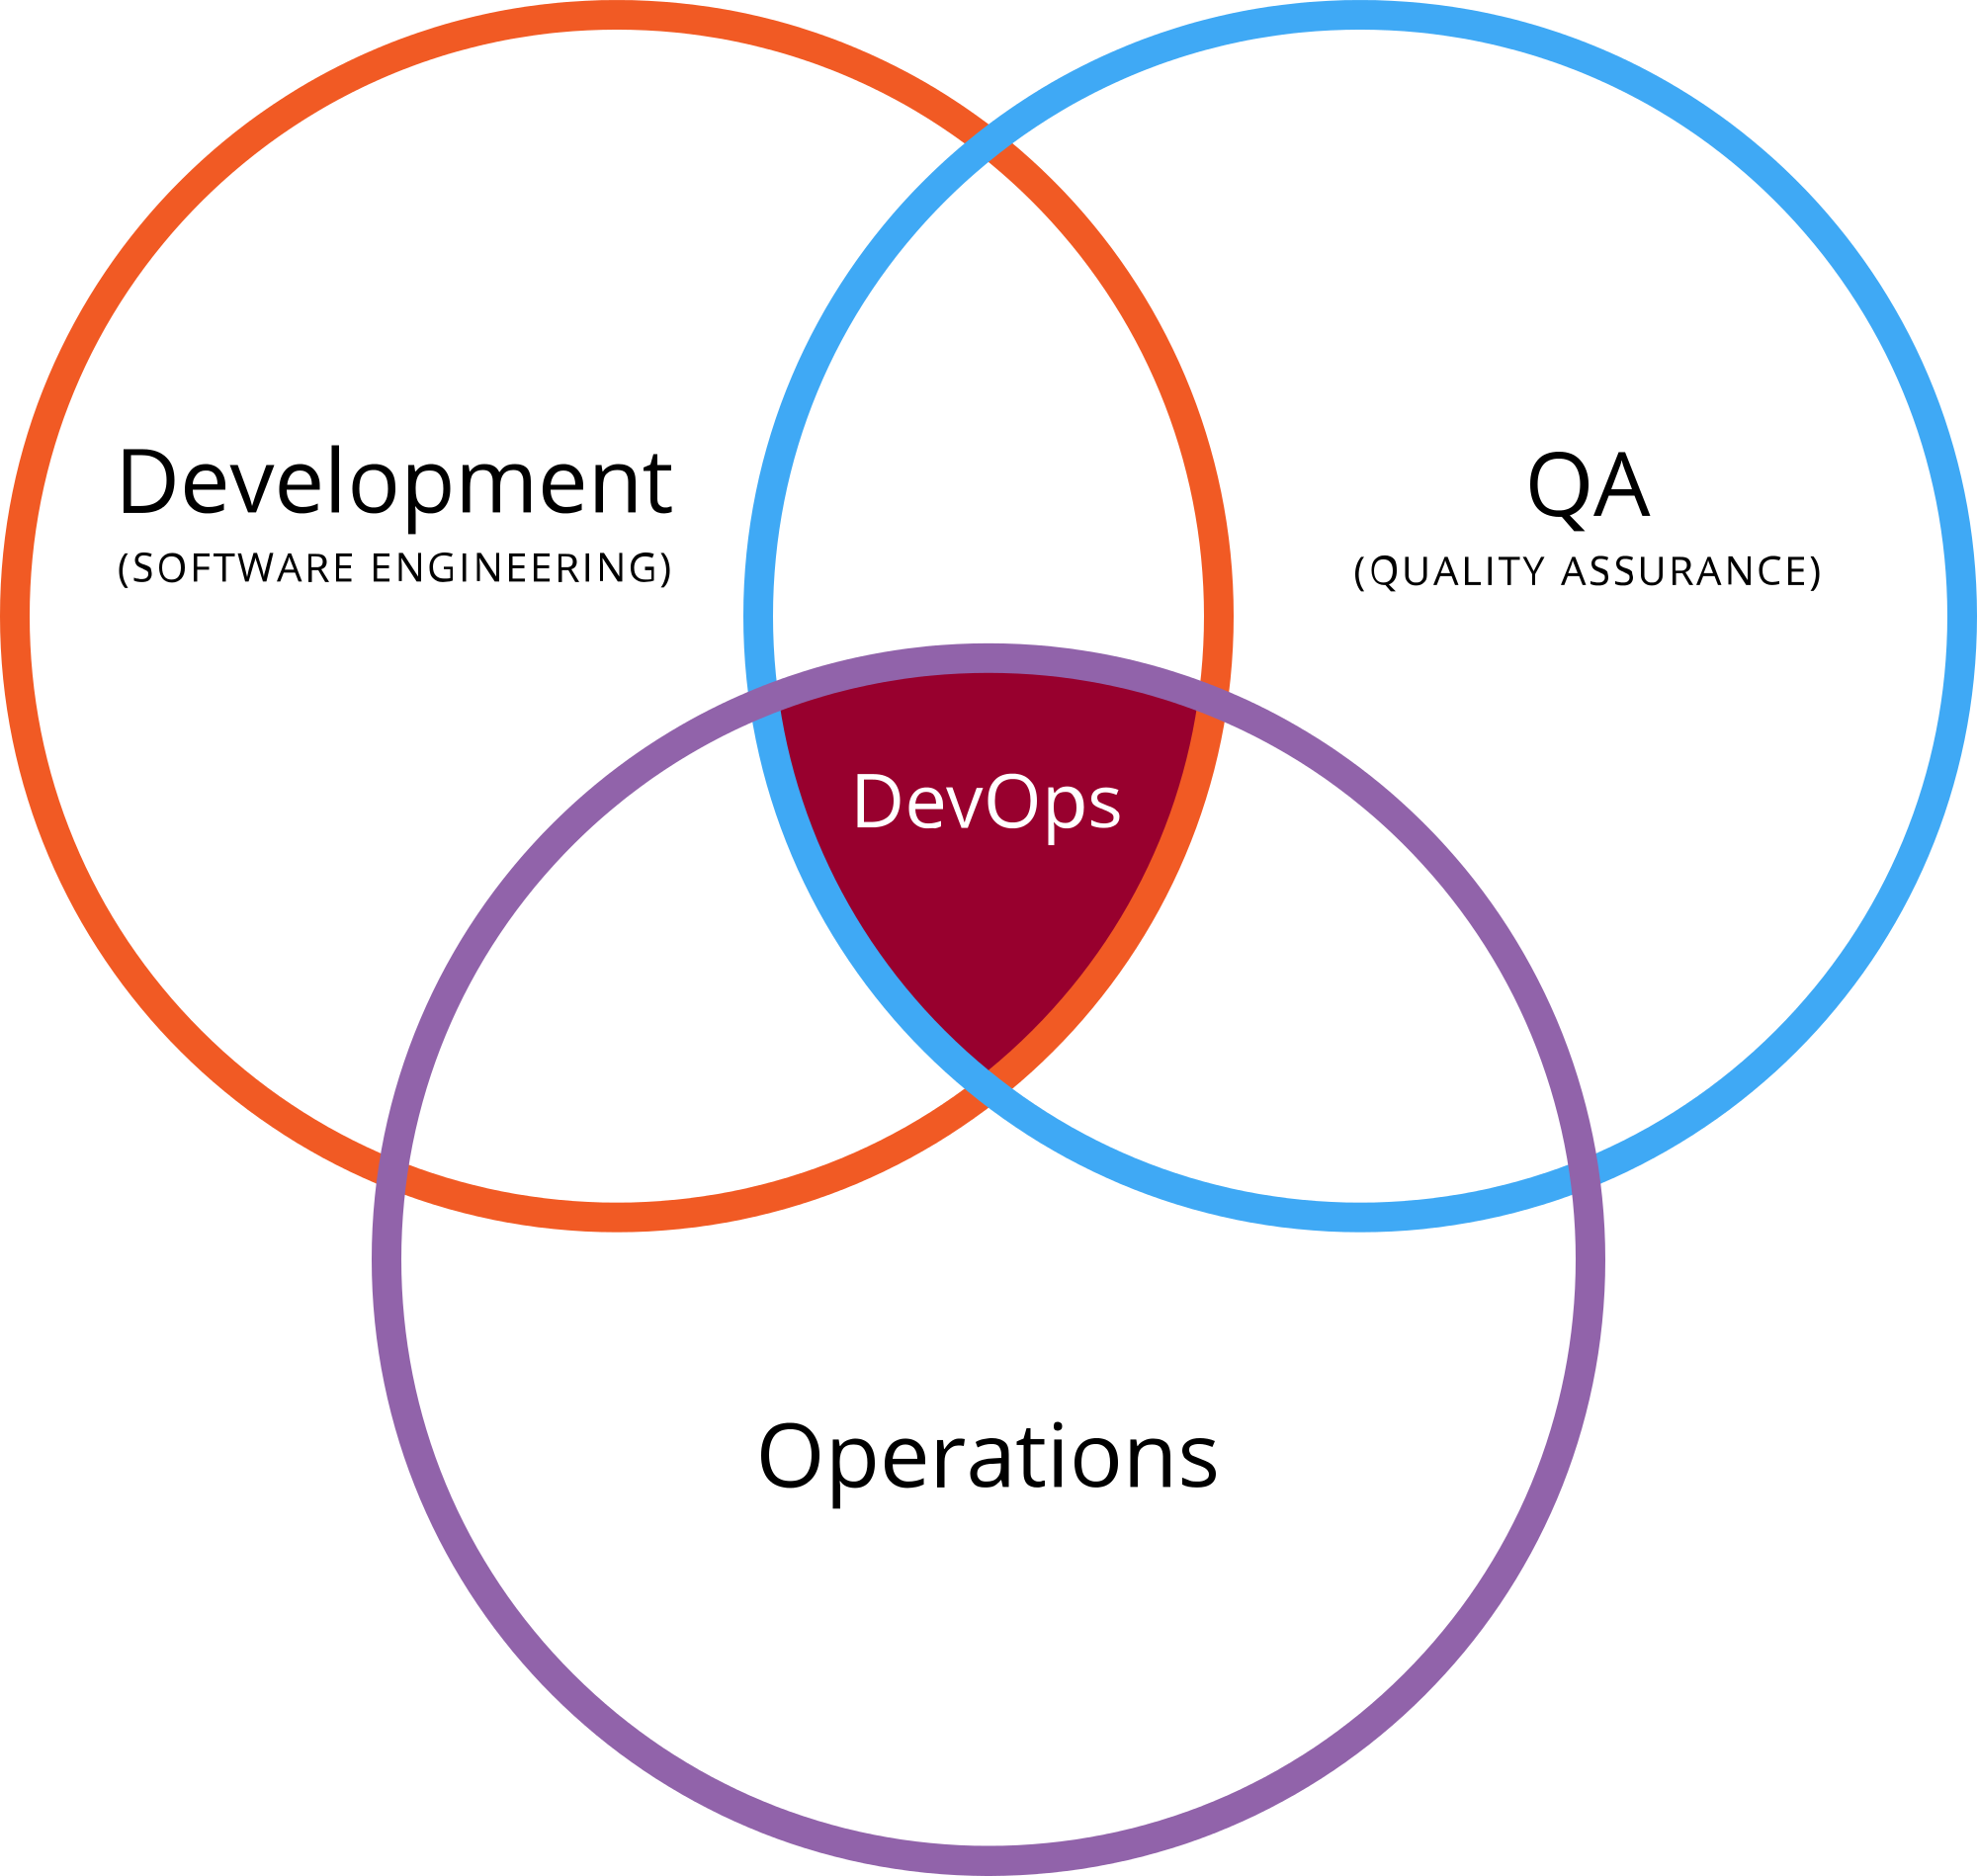
\includegraphics[width=7cm]{Partes_DevOps.png}
\caption{Perfil \ac{DevOps}}
\end{figure}

Por lo que \ac{DevOps} es utilizado para conseguir realizar una entrega continua rápida y de calidad al cliente, para ello, utiliza la integración continua para realizar integraciones frecuentes procurando así obtener siempre un código robusto y estable, tras comprobar que se realiza de manera correcta el \textit{build} del proyecto y se superan las pruebas.

Para conseguir obtener una entrega continua de calidad, tal y como se ha dicho antes, se utiliza la integración continua, pero la integración continua contiene una serie de características y requisitos para que sea realizada de manera correcta.

\section{Características y requisitos de la integración continua}

La integración continua consta de una serie de propuestas (o buenas prácticas) a seguir para que se desarrolle de la mejor manera posible. Entre todas estas propuestas de buenas prácticas destacan las nombradas por Martin Fowler\cite{IC}, precursor de la integración continua.

\clearpage

\begin{enumerate}
\item \textbf{Mantener un único repositorio fuente.}

Los desarrollos de software trabajan sobre archivos que necesitan orquestarse entre sí para realizar el \textit{build} de un producto. 

Rastrearlos supone un esfuerzo, y más, si cada desarrollador tiene fragmentos de código en su equipo local, en distintas carpetas o lugares de almacenamiento lo cual es un error.

Cuándo el proyecto es desarrollado por un equipo de desarrollo formado por varias personas en vez de por una sola, esta situación es inaceptable.

Con lo cual, no supone una sorpresa que con el paso del tiempo los equipos de desarrollo de software hayan construido herramientas que solucionen estos problemas, estas herramientas son conocidas como sistemas de control de versiones, las cuales, en poco tiempo, se han convertido en una parte imprescindible en la gestión de los proyectos de desarrollo de software.

\begin{figure}[!h]
\centering
   
\includegraphics[width=8cm]{Repositorios_SCV.png}
\caption{Repositorios y sistemas de control de versiones}
\end{figure}

Otro error común en equipos que sí utilizan repositorios, consiste en que no ponen todo dentro de él, es decir, contienen parte del código en local y parte del código en repositorios. Es decir, se debe colocar todo lo que sea necesario para hacer un \textit{build} en el repositorio, incluyendo: \textit{scripts} de prueba, archivos de propiedades, esquemas de bases de datos, \textit{scripts} de instalación o bibliotecas de terceros.

%Por lo tanto, se propone implantar un sistema de control de versiones, asegurando así que todo el equipo conozca cual es el lugar para obtener el código fuente, como una buena práctica a la hora de desarrollar un sistema de integración continua.

\item \textbf{Automatizar el \textit{build}.}

Convertir el código fuente en sistemas de ejecución puede ser un proceso complicado que involucra, entre otros muchos pasos, compilación de código, mover archivos o cargar esquemas dentro de las bases de datos\cite{humble2010continuous}. 

Sin embargo, como la mayoría de las tareas en esta parte del desarrollo de software, se puede y se debe automatizar. Ya que realizar estas tareas mediante comandos y de manera manual no es nada más que una pérdida de tiempo y, además, supone una alta probabilidad de cometer errores.

Los entornos automatizados para \textit{builds} son una herramienta común de los sistemas. El mundo UNIX los ha hecho por décadas; la comunidad Java desarrolló Ant, Maven y Gradle, la comunidad .NET desarrolló NAnt y ahora dispone de MSBuild.

Un error típico al desarrollar consiste en no incluir todo en el \textit{build} automatizado. El \textit{build} debe poder obtener del repositorio el esquema de la base de datos y ponerlo en marcha en el entorno de ejecución.

Los \textit{build scripts} se obtienen de diferentes formas y a menudo son particulares para una plataforma o comunidad. Hacer un gran \textit{build} en los \textit{script} lleva tiempo, y no se pretenden realizar todos esos pasos sólo para hacer un pequeño cambio; entonces, una buena herramienta para hacer un \textit{build} analiza lo que necesita cambiar como parte del proceso. La forma más común de hacer esto es comprobar las fechas de la fuente y archivos de objetos y sólo compilar si la fecha de la fuente es posterior. %Las dependencias se pueden convertir en ``tramposas'': si un archivo de objeto cambia lo que depende de él, puede que se necesite volver a rehacer un \textit{build}.

Dependiendo de las necesidades, puede resultar adecuado fragmentar la construcción del software en diferentes artefactos o partes del proyecto. Algunos componentes se pueden construir de forma autónoma. Un \textit{build script} debe permitir hacer un \textit{build} en destinos alternativos para casos diferentes.

%Por lo tanto, se propone como una buena práctica que mediante un comando y de manera automática, se pueda levantar un software y pueda ser utilizado sin necesidad de realizar más acciones.

\item \textbf{Crear \textit{builds} testeables.}

Tradicionalmente, \textit{build} significa compilar y el resto de pasos que se necesiten para lanzar un programa. Un programa puede ejecutarse, pero eso no significa que lo haga de forma correcta. Los lenguajes modernos, en especial los tipados de manera estática, pueden atrapar muchos \textit{bugs}, pero otros \textit{bugs} permanecen ocultos.

Una forma de encontrar \textit{bugs} de manera más rápida y eficiente es incluir pruebas automatizadas en el proceso de \textit{build}. Estas pruebas no son perfectas al 100\%, pero pueden descubrir muchos \textit{bugs}; por lo que son útiles.

Un código autotestable es aquel que tiene un número representativo de pruebas que permiten comprobar una gran parte del código. Las pruebas deben poder dispararse desde un comando simple y autocomprobarse. El resultado de la ejecución del conjunto de pruebas debe indicar si alguna prueba ha fallado.

Por otra parte, se afirma que mediante estas pruebas no se descubrirán todos los \textit{bugs}. Por lo que, estas pruebas no implican la ausencia de \textit{bugs} en el código fuente.

Sin embargo, la perfección a la hora de realizar las pruebas no es el único punto que justifica la realización de un \textit{build} que sea capaz de testearse.

Tal y como dice Martin Fowler\cite{IC} de manera coloquial: ``\textit{La ejecución de pruebas que no manifiestan todos los errores de un código con frecuencia, son mucho mejores que la ejecución de aquellas pruebas perfectas que nunca se escribieron}''.

%Por lo tanto, se propone como una buena práctica que los \textit{builds} sean capaces de testearse asimismos, puediendo así, encontrar errores que hayan pasado inadvertidos.
\clearpage

\item \textbf{Todos hacen \textit{commit} al \textit{mainline} todos los días.}

La integración continua es, ante todo, comunicación. La integración continua permite a los desarrolladores contar al resto de desarrolladores los cambios que han realizado. La comunicación continua permite que el resto del equipo conozca los cambios que se han realizado.

El único prerrequisito para un desarrollador que hace \textit{commit} al \textit{mainline} es que el resto de desarrolladores puedan hacer un \textit{build} correcto del código. Esto, por supuesto, incluye superar de manera correcta la pruebas que contenga el \textit{build}.

Al realizar el ciclo completo para hacer \textit{commit} de manera frecuente, los desarrolladores descubren rápidamente si existe algún conflicto entre el código desarrollado por dos o más desarrolladores distintos. La clave para solucionar problemas de forma rápida es encontrar dicho problema de manera rápida. Con desarrolladores que hacen \textit{commit} cada pocas horas, el conflicto se puede detectar dentro de las primeras horas, es decir, el error no ha tenido tiempo de propagarse por lo que, de manera rápida, se soluciona. Los conflictos y errores que no son detectados rápidamente son difíciles de resolver cuando se descubren.

\begin{figure}[!h]
\centering
   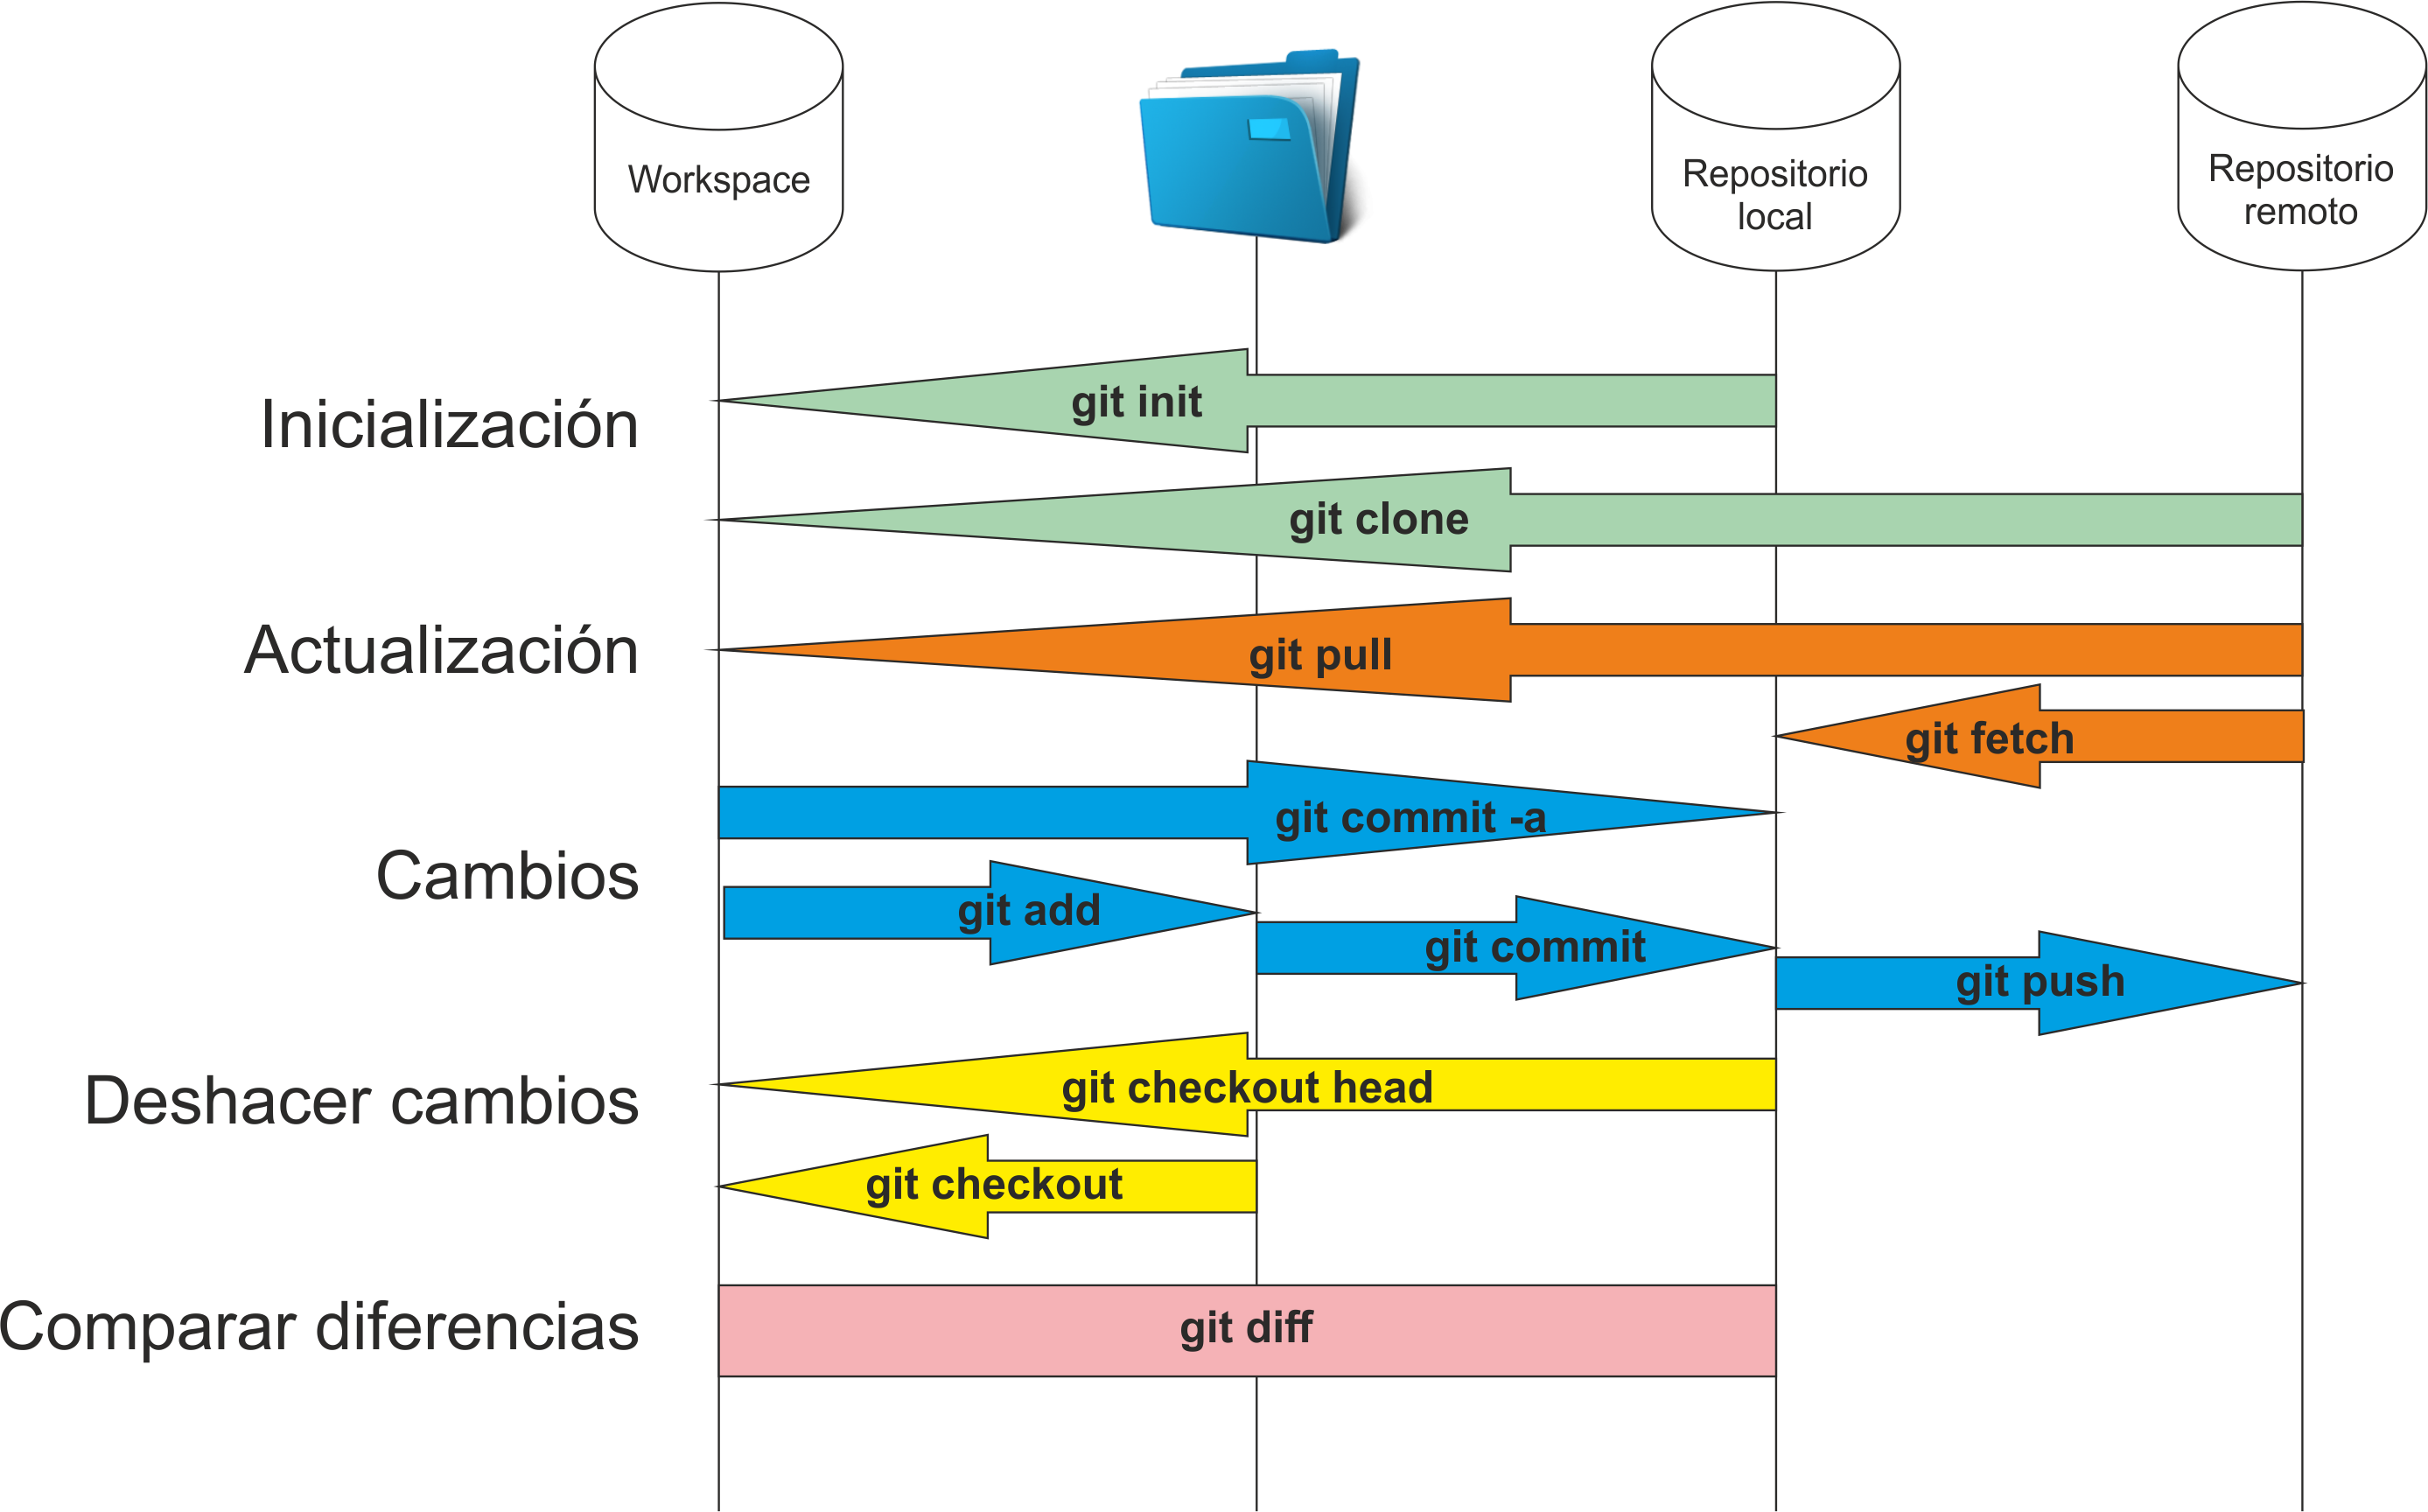
\includegraphics[width=13cm]{Flujo_Git.png}
\caption{Algunas acciones de Git\cite{Git_Manual}.}
\end{figure}

El hecho de realizar un \textit{build} cuando se actualiza la copia de trabajo local significa que se han detectado conflictos en la compilación. Como el \textit{build} tiene la capacidad de testearse asimismo, también detecta conflictos en la ejecución del código.

\clearpage

Como sólo hay un par de horas de cambios entre \textit{commits}, no hay muchos lugares donde pueda estar escondido el problema, por lo que se encuentra el error y se soluciona de manera rápida. Además, el proyecto que se está desarrollando no ha cambiado mucho dado que ha transcurrido poco tiempo, por lo que se puede \textit{debuggear} para ayudar a encontrar el error.

%Por lo tanto, se propone como una buena práctica que los desarrolladores hagan \textit{commit} al \textit{mainline} de manera frecuente, mínimo una vez al día, aunque lo ideal sería que se realizase con más frecuencia, para mantenerlo fuerte y actualizado.

\item \textbf{Hacer \textit{commit} debe construir el \textit{mainline} en una máquina de integración.}

Haciendo \textit{commits} a diario, se obtienen \textit{builds} probados con mucha frecuencia. Por lo que el \textit{mainline} permanece en estado saludable. Sin embargo, aún el desarrollo no es perfecto y siguen surgiendo errores. Una razón es la disciplina, el desarrollador debe actualizar y hacer un \textit{build} antes de hacer \textit{commit}, para comprobar que el proceso de hacer \textit{commit} se ha realizado de manera correcta hasta el final.

Como resultado se debe asegurar que los \textit{builds} se realicen en una máquina de integración y sólo si este \textit{build} de integración se realiza con éxito se debe hacer \textit{commit} al \textit{mainline}. Se debe monitorizar el \textit{build} del \textit{mainline} para poder repararlo en caso de que se rompa

%El resultado de esto es que no debes abandonar el \textit{commit} realizado hasta que el \textit{build} de \textit{mainline} haya sido realizado incorporado con éxito junto con los últimos \textit{commits} que se hayan agregado. 

Hay dos maneras para asegura que se ha realizado este proceso de manera correcta: utilizar un \textit{build} manual o un servidor de integración continua.

Utilizar un \textit{build} manual es simple. Esencialmente, consiste en un \textit{build} que se realiza en el repositorio antes que el \textit{commit}.%, se dirige a la máquina de integración, se hace un \textit{checkout} del \textit{head} del \textit{mainline} (que ahora contiene su últimos \textit{commits}) y comienza el \textit{build} de integración. Se monitoriza el progreso y si se completa con éxito se hace \textit{commit}.

Un servidor de integración continua actúa como un monitor del repositorio. Cada vez que finaliza un \textit{commit} contra el repositorio, el servidor automáticamente realiza un \textit{checkout} de las fuentes en la máquina de integración, inicia un \textit{build}, y notifica los resultados obtenidos del \textit{build} al desarrollador que ha realizado el \textit{commit}, el \textit{build} no termina hasta que se obtiene la notificación.

Muchas organizaciones realizan \textit{builds} regulares en un cronograma programado, por ejemplo, todas las noches. Pero no se obtienen los mismos resultados, puesto que no es igual que un \textit{build} continuo y no es suficiente para ser considerado como integración continua.

La finalidad de la integración continua es encontrar problemas tan pronto como sea posible. Un \textit{build} nocturno significa que los \textit{bugs} estuvieron alojados durante todo el día en el código sin ser detectados. Una vez que están en el sistema por tanto tiempo, lleva mucho tiempo encontrarlos y solucionarlos.

%Por lo tanto, se propone como una buena práctica que los desarrolladores hagan \textit{commits} de manera frecuente, pero realizan el \textit{build} del proyecto para comprobar que sus cambios han sido integrados correctamente en la máquina de integración y que no permanecen errores albergados en el código durante mucho tiempo.

\clearpage 

\item \textbf{Mantener rápido el build.}

El objetivo de la integración continua es proporcionar un \textit{feedback} rápido. %La peor actividad o práctica posible dentro de la integración continua consiste en un \textit{build} que tarde mucho tiempo en realizarse. 

Para aquellos proyectos, según \ac{XP}, en los que su \textit{build} tarde un máximo de 10 minutos en realizar todo sus pasos, son considerados \textit{builds} con un tiempo óptimo de construcción, actualmente, la mayoría de proyectos logran no superar ese tiempo.

Se considera de gran valor para un proyecto realizar un esfuerzo para lograr reducir el tiempo de construcción del \textit{build}, puesto que cada minuto que se reduzca en la realización del \textit{build} es un minuto más para cada desarrollador cada vez que haga \textit{commit}. Puesto que la integración continua demanda hacer \textit{commits} con alta frecuencia esto implica ahorrar una gran cantidad de tiempo.

Por lo tanto, realizar un \textit{build} que se ejecute en poco tiempo supone reducir el tiempo en el cual un proyecto finalice.

%Probablemente, el paso crucial es comenzar a trabajar en la configuración de un \textit{pipeline} de \textit{deployment}. La idea de un \textit{pipeline} de \textit{deployment} consiste en tener la capacidad para realizar múltiples \textit{builds}. El \textit{commit} al \textit{mainline} activa el primer \textit{build}, también conocido como ``el \textit{build} de \textit{commit}''. ``El \textit{build} de \textit{commit}'' es el \textit{build} que tiene que realizarse más rápido, y como consecuencia, tendrá una serie de accesos directos que reducirán la capacidad de detectar errores. Con ello, se persigue balancear la necesidad de encontrar \textit{bugs} y la velocidad, así un buen \textit{build} de \textit{commit} es lo suficientemente estable para que otras personas trabajen en él y al mismo tiempo de encontrar errores.

%Por lo tanto, se propone como una buena práctica que los desarrolladores desarrollen y realicen \textit{builds} que sean capaces de realizarse en poco tiempo y tengan la capacidad de encontrar errores para ser reportados a los desarrolladores.

\item \textbf{Prueba en un clon del entorno de producción.}

Cuando se realizan pruebas se persigue un objetivo, que consiste en eliminar, bajo condiciones controladas, cualquier problema que surja durante la ejecución del \textit{build}.

Para conseguir este objetivo, obtiene un gran peso el entorno dentro del cual el \textit{build} se ejecutará. Como resultado, se pretende configurar el entorno de prueba para que sea lo más parecido a un clon del entorno de producción donde será ejecutado ese \textit{build}, utilizando el mismo software de base de datos (incluyendo las mismas versiones), la misma versión de sistema operativo, colocando todas las bibliotecas o recursos que sean necesarios donde se encontrarían en el entorno de producción dentro del entorno de prueba, aunque no sean necesarias también se recomienda utilizar las mismas direcciones IP, en los mismos puertos y ejecutándose en el mismo hardware.

Cualquier desarrollador de software, conoce que no es posible probar en un clon de cada una de las posibles computadoras con todo el software de terceros que diferentes personas estén ejecutando. Ocurre lo mismo con algunos entornos de producción que pueden ser muy costosos de duplicar. Más allá de estos límites, el objetivo debe seguir siendo duplicar el entorno de producción tanto como sea posible, y entender los riesgos que aceptas para cada diferencia entre la prueba y la producción.

%Por lo tanto, se propone como una buena práctica que las pruebas realizadas a cualquier código desarrollado sean realizadas en un clon del entorno de producción.

\item \textbf{Facilitar la obtención del último archivo ejecutable.}

Desarrollar software no es sencillo, una de las partes más difíciles del desarrollo de software consiste en asegurar que se está realizando un \textit{build} correcto.

Cualquier desarrollador involucrado en un proyecto de software debería poder obtener el archivo ejecutable más reciente y poder ejecutarlo: para demostraciones, pruebas, u observar qué ha cambiado en el desarrollo sin tener que realizar ningún cambio en su máquina o en el \textit{build}.

%Por lo tanto, se propone como una buena práctica que dentro del repositorio común se encuentre el último archivo ejecutable desarrollado.

\item \textbf{Todo el equipo debe observar los cambios que están sucediendo.}

La integración continua, como ya se ha dicho en varias ocasiones, es comunicación, así que se debe asegurar de que todos los miembros del equipo puedan ver fácilmente el estado del sistema y los cambios que se han realizado en él\cite{dybaa2008empirical}.

%Muchos equipos, mediante la conexión de una pantalla continua, monitorizan el estado y el sistema del \textit{build}, y con simples códigos como: luces verdes si el \textit{build} funciona o rojas si falla, permiten que todo el equipo conozca lo que está sucediendo y el estado en el que se encuentra el \textit{build}.

Si se utiliza la integración continua manual, la visibilidad sigue siendo esencial. El monitor de la máquina física del \textit{build} debe mostrar el estado del \textit{build} del \textit{mainline}.

Por ello, surge la ventaja de utilizar un sitio web, ya que así, aquellos que no están en el mismo lugar, pueden conocer el estado del proyecto accediendo a una página web.

%En general, se considera más óptimo y eficiente que todo el equipo de desarrollo de un proyecto se encuentre trabajando activamente en el mismo lugar, pero, por diferentas situaciones y motivos, hay miembros del equipo que no se encuentran junto al resto del equipo.

%Por lo tanto, se propone como una buena práctica que, mediante el medio que se desee, cualquier miembro del equipo de desarrollo de un proyecto sea capaz de conocer los cambios realizados o el estado en el que se encuentra el proyecto.

\item \textbf{Automatizar el \textit{deployment}.}

Para ser capaz de realizar una integración continua de manera correcta se necesitan múltiples entornos: un entorno para ejecutar pruebas de \textit{commit}, uno o más entornos para ejecutar pruebas secundarias, etcétera.

Además, si se necesitan mover archivos ejecutables entre los diferentes entornos varias veces al día y de manera repetitiva, no se puede realizar de manera manual dado que es ineficiente y supone pérdidas de tiempo, por lo que se hace necesario automatizar el proceso.

En consecuencia, también se necesitan \textit{scripts} que permitan realizar el \textit{deployment} en el entorno de producción con facilidad. No se realiza el \textit{deployment} de una producción cada día, pero el \textit{deployment} automático permite acelerar el proceso y reducir la capacidad de cometer errores.

%Por lo tanto, se propone como una buena práctica la necesidad de automatizar el \textit{deployment} de un proyecto para reducir la capacidad de cometer errores y acelerar el proceso.

\end{enumerate}


\section{Herramientas}

\subsection{Bamboo}

Bamboo es una herramienta contenida en un contenedor web, posee licencia de propietario, tiene compatibilidad con varios \textit{builders} de Windows como MSBuild, NAnt y Visual Studio, además, también cuenta con \textit{builders} de Java, tales como Ant y Maven, permite el envío de notificaciones vía email, Google, XMPP y RSS. Integrado con varios \ac{IDE} como IntelliJ IDEA, Eclipse y Visual Studio. Destaca también su integración con Bitbucket y GitHub.

\subsection{CircleCI}

CircleCI\cite{CircleCI} es un software de integración continua que está contenido en un \textit{hosted}, con licencia ``\textit{Creative Commons}'', tiene compatibilidad con Python, Ruby y Java entre otros, se encuentra disponible para Ubuntu y macOS. Se integra con repositorios como GitHub y Bitbucket o con herramientas como Azure y Docker, permite enviar notificaciones mediante Jira y Slack.

\subsection{Jenkins}

Al igual que Bamboo esta herramienta está contenida en un contenedor web, sin embargo, es una herramienta de software libre ya que cuenta con licencias de “\textit{Creative Commons}” y “\textit{MIT}”, contiene MSBuild y NAnt, \textit{builders} de Windows y Ant, Maven y Kundo, \textit{builders} de Java, Ruby, Python y shell script. Permite enviar notificaciones vía Twitter, Google, email, Android o Slack. Posee compatibilidad con varios \ac{IDE}, Eclipse, IntelliJ IDEA y NetBeans, además también cuenta con la integración de Google Code, Jira, Bitbucket, GitHub, GitLab y Redmine entre otras muchas.

\begin{figure}[!h]
\centering
   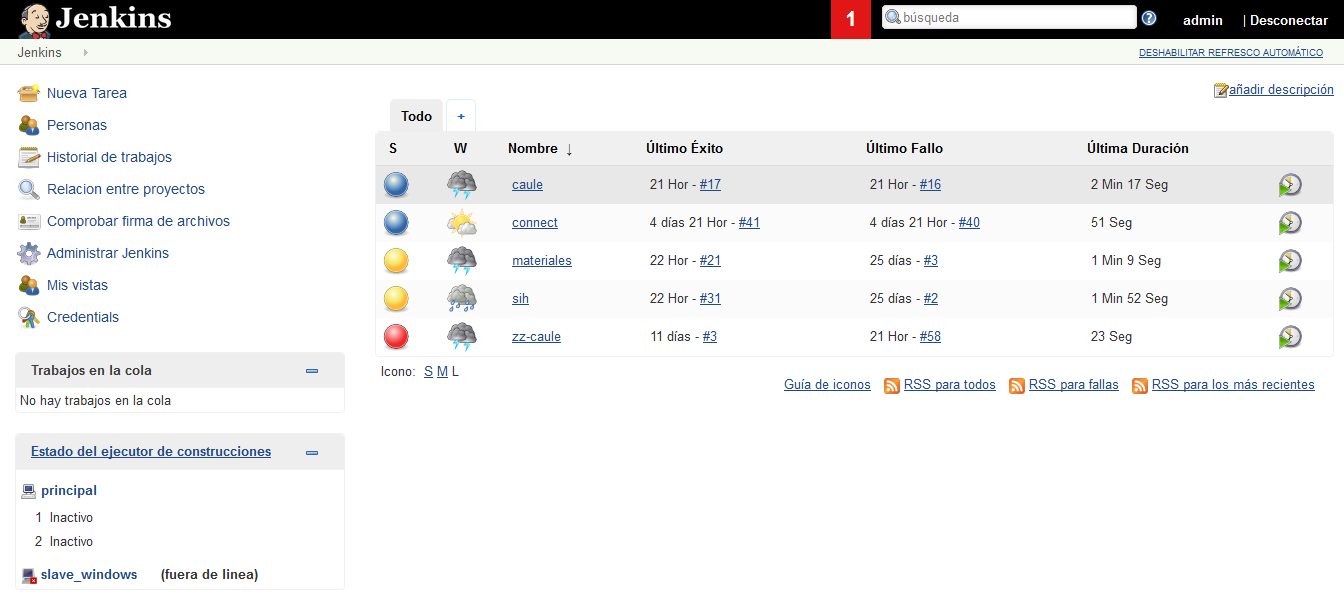
\includegraphics[width=16cm]{PanelPrincipal_Jenkins.PNG}
\caption{Panel principal de Jenkins}
\end{figure}

\subsection{Solano CI}

Esta herramienta se encuentra albergada en un \textit{hosted}, en la nube privada o sobre software multiplataforma, posee licencia de propietario, no cuenta con \textit{builders} para Windows, posee \textit{builders} de Java para Ant, Andriod, Maven y Gradle y otros \textit{builders} para C, C++, JavaScript, PHP o Ruby. Cuenta con notificaciones vía email, pero no cuenta con integración para \ac{IDE}, sin embargo, sí se encuentra integrada con GitHub o Bitbucket.

\subsection{TeamCity}

Al igual que Bamboo y Jenkins está contenida en un contenedor web, posee licencia de propietario, cuenta con \textit{builders} de Windows tales como MSBuild, NAnt y VisualStudio, \textit{builders} de Java tales como Ant, Maven y Gradle, notificaciones vía email, XMPP y RSS, compatible con \ac{IDE} como Eclipse, Visual Studio o IntelliJ IDEA.

\clearpage

\subsection{Travis CI}

Travis CI se alberga en un \textit{hosted}, su licencia es "\textit{MIT}", no posee \textit{builders} para Windows pero sí para Java, donde destacan Ant, Maven y Gradle, además, soporta \textit{builders} para C, C++, Go, Groovy, Python, Ruby o PHP. Permite enviar notificaciones vía email o Slack entre otros medios, pero no posee integración con \ac{IDE}, pero sí con GitHub.

\begin{figure}[!h]
\centering
   
\includegraphics[width=8cm]{Logos_CI.jpg}
\caption{Herramientas de integración continua}
\end{figure}


\subsection{Comparativa}

\begin{center}
\rowcolors{1}{gray!25}{white}
\begin{longtable}{p{.30\textwidth} p{.30\textwidth}}
\hline \hline
  \textbf{Herramienta} & \textbf{Tipo de licencia} \\
    \hline \hline
    Bamboo & Propietario\\
    \hline\hline
    CircleCI & \textit{Creative Commons}\\
    \hline\hline
    Jenkins & \textit{Creative Commons} y \textit{MIT}\\
    \hline\hline
    Solano CI & Propietario\\
    \hline\hline
    TeamCity & Propietario\\
    \hline\hline
    Travis CI & \textit{MIT}\\
    \hline\hline    
    
\caption{Comparativa de tipo de licencia}
\end{longtable}
\end{center}

\clearpage

\begin{center}
\rowcolors{1}{gray!25}{white}
\begin{longtable}{p{.30\textwidth} p{.30\textwidth}}
\hline \hline
  \textbf{Herramienta} & \textbf{\textit{Hosting}} \\
    \hline \hline
    Bamboo & Contenedor web\\
    \hline\hline
    CircleCI & \textit{Hosted}\\
    \hline\hline
    Jenkins & Contenedor web\\
    \hline\hline
      Solano CI & Contenedor web\\
    \hline\hline
    TeamCity & Contenedor web\\
    \hline\hline
    Travis CI & \textit{Hosted}\\
    \hline\hline    
    
\caption{Comparativa de \textit{hosting}}
\end{longtable}
\end{center}

\begin{center}
\rowcolors{1}{gray!25}{white}
\begin{longtable}{p{.30\textwidth} p{.30\textwidth}}
\hline \hline
  \textbf{Herramienta} & \textbf{Notificaciones} \\
    \hline \hline
    Bamboo & Email, Google, XMPP y RSS\\
    \hline\hline
    CircleCI & Jira y Slack\\
    \hline\hline
    Jenkins & Twitter, Google, email,
Android y Slack\\
    \hline\hline
      Solano CI & Email\\
    \hline\hline
    TeamCity & Email, XMPP y RSS\\
    \hline\hline
    Travis CI & Email y Slack\\
    \hline\hline    
    
\caption{Comparativa de envío de notificaciones}
\end{longtable}
\end{center}

\clearpage

\begin{center}
\rowcolors{1}{gray!25}{white}
\begin{longtable}{p{.30\textwidth} p{.30\textwidth}}
\hline \hline
  \textbf{Herramienta} & \textbf{\textit{Builders}} \\
    \hline \hline
    Bamboo & MSBuild, NAnt, Vistual Studio, Ant y Maven\\
    \hline\hline
    CircleCI & Python, Ruby, Ant y Maven\\
    \hline\hline
    Jenkins & MSBuild, NAnt, Ant, Maven, Gradle, Android, Kundo, Ruby, Python y Shell script\\
    \hline\hline
      Solano CI & Ant, Android, Maven, Gradle, C, C++, JavaScript, PHP y Ruby\\
    \hline\hline
    TeamCity & MSBuild, NAnt, Visual Studio, Ant, Maven y Gradle\\
    \hline\hline
    Travis CI & Ant, Maven, Gradle, C, C++, Go, Groovy, Python y Ruby\\
    \hline\hline    
    
\caption{Comparativa de \textit{builders}}
\end{longtable}
\end{center}

\clearpage

\begin{center}
\rowcolors{1}{gray!25}{white}
\begin{longtable}{p{.30\textwidth} p{.30\textwidth}}
\hline \hline
  \textbf{Herramienta} & \textbf{Otras integraciones} \\
    \hline \hline
    Bamboo & IntelliJ IDEA, Eclipse, Visual Studio, Bitbucket y GitHub\\
    \hline\hline
    CircleCI & Azure y Docker\\
    \hline\hline
    Jenkins & Eclipse, IntelliJ IDEA, NetBeans, Google Code, Jira, Bitbucket, GitHub, GitLab y Redmine\\
    \hline\hline
      Solano CI & GitHub y Bitbucket\\
    \hline\hline
    TeamCity & Eclipse, Visual Studio y IntelliJ IDEA\\
    \hline\hline
    Travis CI & GitHub\\
    \hline\hline    
    
\caption{Comparativa de integraciones extras}
\end{longtable}
\end{center}